% !TEX root = ../main.tex


\section{Introductory Remarks}




%decentralized exchanges allow the market participants to be fully authoritative over their assets using their private keys. 
%One issue with decentralized 
%
%Cryptocurrency trading on centralized exchanges has been shown to be vulnerable to cybersecurity hacking and internal frauds over the years, with the most infamous hacks being Mt. Gox and Coincheck. In addition, trading on centralized exchanges is not compatible with DeFi applications since it is technically infeasible to bridge between decentralized applications and centralized servers without compromising the trust model.







% = = = = = = = = = = = = = = = = = = = = = = = = = = = = = = = = = = = = = = = = = =

\section{Order Books}

Order books are data structures that maintain lists of bid and ask orders for various assets (\eg currencies, stocks, bonds \etc) in specific markets. The most common version of order books is what we call a \textit{double auction}, where market participants submit their bid and ask orders and the market clearing price will be calculated as the average between the best bid and best ask prices. Order books often sort orders based on their price and submission time (this order allocation technique is called price-time priority)~\cite{preis2011price}, where orders are prioritized from highest price to lowest and given any two orders with the same price, they will be sorted based on their submission timestamps.

\par

Looking more closely, order books are rather electronic ledgers that get updated over time. Given the definition of the Ethereum blockchain, that is a distributed ledger, the idea of implementing an order book in the form of a smart contract will seemingly resolve the existing issues with centralized exchanges. However, this design is not feasible due to some crucial challenges that exist within blockchains:

\begin{itemize}

\item \textbf{Speed.}

\item \textbf{Front-running and Censorship.}

\item \textbf{Enforcing Time.}

\end{itemize}


% = = = = = = = = = = = = = = = = = = = = = = = = = = = = = = = = = = = = = = = = = =






% = = = = = = = = = = = =Notes Discussed in Meetings = = = = = = = = = = = = =  %

% Our two competitors are Uinswap and Loopring (that uses ZK roll ups):
% 	1- Uniswap: we can argue that in traditional markets we have various traditional exchanges. Each of these exchanges have different trading rules and designs which work for different traders.
%	2- Loopring:
%		2-1: Barrier to entry: In order for a trader to trade specific ERC20 on Loopring, Loopring has to agree to support that token. It might not be difficult and they probably approve the token as long as it is standard compliant.
%		2-2: ZK proofs are quick and cheap to verify but they are expensive and time consuming to generate: (1) now they are generating these proofs for free but later they charge traders for doing that. (2) Looping does not probably generate these proofs per every block so the settlement and 				clearing is not happening per block. So we have faster clearing and settlement as we clear everything per block. 
% 		2-3: Loopring is non-custodial, meaning that the money moves only when the proofs come, so there is a latency in transferring funds to the traders.


% The heap with dynamic array can do 26 pairs of matches at worst case matching whereas Linkedliat does 90 pairs. So if we want to cap the orders over 4 PQs, we’re basically increasing the heap size which makes match more expensive for nothing (every time a match happens and the root is deleted the whole heap is reheapified)

% There will be no ties as we use 2 counters for buy and sell orders. These counters are concatenated them with the price. So we somehow enforce time priority


% = = = = = = = = = = = = = = = = = = = = = = = = = = = = = = = = = = = = = = = = = = = = = = = = = = = = = = = = = = = = = = = = = = = = =  %

% = = = = = = = = = = = =Clearing Mappings = = = = = = = = = = = = =  %
\section{Clearing Mappings}

To facilitate a safe exchange among buyers and sellers, we implement the CallMarket smart contract in the form of a \textit{collateralized}; for market participants to be able to send bid and/or ask orders, they have to first supply assets (depending on what asset they aim to trade) as collaterals  by calling any of the  \texttt{DepositToken()} or \texttt{DepositEther()} methods. The collateralized CallMarket acts as a payment guarantees and market participants cannot default on payment or delivery of their assets.

To maintain the collateral balance of each market participant, we use two Solidity type one-to-one mapping that map Ethereum addresses to 256 bits unsigned integers; \texttt{TotalBalance} and \texttt{UnavailableBalance}. Once market closes and orders are matched, the \texttt{UnavailableBalance} needs to be cleared. However, since it is not possible to delete the entire mapping without knowing the keys~\footnote{https://solidity.readthedocs.io/en/v0.5.12/security-considerations.html}, clearing the \texttt{UnavailableBalance} mapping remains a challenging issue to solve . Here we provide a landscape of solutions for that.
%only individual keys and what they map to can be deleted.

\begin{enumerate}

\item \textbf{Creating a New Mapping Every Time the Market Opens.} Instead of clearing the \texttt{UnavailableBalance} of traders at the end of a matching process, we could create a new mapping every time the market opens. Note that using this solution, traders can only claim their funds (using the \texttt{ClaimEther()} and/or \texttt{ClaimToken} methods) only when the market is in state \texttt{Closed}. 

\item \textbf{Creating Custom Keys for the Mapping.} We can create custom keys for the mapping by defining a counter as a global variable inside the CallMarket smart contract. This counter is incremented at the end of the matching process. So instead of clearing the mapping, we only use another portion of it every time the market opens.

\item \textbf{Storing the Mapping in a Data-Contract.} Another design proposal is to create a smart contract every time the market opens, this data contract only stores the \texttt{UnavailableBalance} mapping and will be killed at the end of the matching process.

\item \textbf{Storing the Mapping keys in additional Array.} Another common pattern is to create an additional array on top of the mapping and iterate over that. This array (\eg address[]) stores the traders' addresses and enables us to iterate over the mapping and delete individual keys and what they map to at the end of the matching process. Not that this is a gas-costly design pattern as we would need to maintain a secondary data structure.

\end{enumerate}

% = = = = = = = = = = = = = = = = = = = = = = = = = = = = = = = = = = = = = = = = = = = = = = = = = = = = = = = = = = = = = = = = = = = = =  %

% = = = = = = = = = = Design Details of PQs = = = = = = = = = = = = = = %
\section{Design Details of PQs}


%= = = = = =Mapping with Keys Stored in Heap = = = = = = =%

\subsection{Mapping with Keys Stored in a Heap}\label{sec:mapping_heap}

To store the orders, here we use Solidity mapping that map orders' ids (256-bit integers) to order structs with their variables of different types. The mapping keys are then stored in a sorted heap that is implemented with a dynamic storage array. Every time a trade happens; (i) the mapping keys associated with the best bid and ask orders are deleted from the heap and the heap is re-sorted, and (ii) the mapping elements containing the best bid and ask orders are deleted from storage completely which refund 15000 gas~\cite{wood2014ethereum}. Deleting the mapping elements is yet a gas-costly operation which lowers down the maximum number of orders the \texttt{Match()} function could handle in this case.~\footnote{Every order structs contains multiple variables of different types and removing them from storage is identical to setting multiple variables to zero.} However, we clear the mapping element once a trade happens in our design as leaving unnecessary data is not a proper design practice.

%= = = = = =Linkedlist = = = = = = =%
 
\subsection {Linkedlist}
Every time a trade happens, we use the \texttt{self-destruct} operation to remove the nodes (\ie smart contracts) containing the best bid and ask orders from the Ethereum blockchain. When a node is deleted, it transfers its funds (if any) to the payable address of the CallMarket contract that has been previously passed to it as a constructor argument. Also, removing a smart contract from the Ethereum blockchain refunds 24000 gas to the caller.

%= = = = = =Linkedlist with Mapping = = = = = = =%

\subsection {Linkedlist with Mapping}
Every time a trade happens when the \texttt{Match()} function is executed, the best bid and ask orders need to be removed from the data structures. We could do this in two different ways; (i) update the head and tail pointers of the linkedlist and/or (ii) removing the mapping elements that contain the best bid and ask orders from storage completely as well as updating the pointers of the linkedlist. \par

For the same reason we mentioned in~\ref{sec:mapping_heap}, we clear the best bid and ask order structs from the mapping every time a trade happens as well as updating the pointers.



% = = = = = = = = = = = = = = = = = = = = = = = = = = = = = = = = = = = = = = = = = = = = = = = = = = = = = = = = = = = = = = = = = = = = =  %

% = = = = = = = = = = = =Closing and Reopening the Market = = = = = = = = = = = = =  %

\section{Closing and Reopening the Market}

% We use one-shot market for the sake of our performance tests on different datastructures. and once we have all the numbers we can think about iterated market.

At the end of the trading period, the market needs to be closed and reopened. However, there is no automatic process to called an Ethereum function and contracts can only run when a function is called. 

%when to close the market?
%What time period?


% = = = = = = = = = = = =How to enforce time on on the Ethereum blockchain? = = = = = = = = = = = = =  %

\subsection{Enforcing Time on the Blockchain}

% We want the market to run on a periodic schedule => it is difficult for market participants to call the \texttt{Close()} function periodically.

% However there are incentives for them to do so: (i) they get paid and refunded (financial incentives), and (ii) Closing the market allow market participants to open it again and start their trading activities

% Another solution pattern to enforce the time is to use the Ethereum Alarm Clock 


% = = = = = = = = = = = =Who Pays the Cost for Closing and Reopening the Market?= = = = = = = = = = = = =  %

\subsection{Who Pays the Cost for Closing and Reopening the Market?}

%%%%% Mahsa: Add whatever was discussed in the meeting %%%%% 


We think it is useful to explore the landscape of possible designs for closing the market. 

\begin{enumerate}

%= = = = = = Miners Close the Market = = = = = = =%

%Jeremy: Miner could close the market as they get paid and the amount could be more than running the function. 
\item \textbf {Miners Close and Reopen the Market.} The difference between the best bid and ask prices is called the \textit{bid-ask spread}. In our design, when the trade occurs between the the highest bid (the highest amount a buyer is willing to pay for an asset) and lowest ask (the lowest amount a seller is willing to accept for an asset) orders, the bid-ask spread is paid to the miner. In addition to this, a miner could close the market and get refunded. The refund amount could be potentially higher than the bid-ask spread which provides enough economic incentives for the miner to execute the \texttt{Close()} function.


% = = = = = = = = = =Processing Orders in Groups= = = = = = = = = = = = = = = %
% Mahsa: Title is good or needs to be changed?

\item \textbf{Processing Orders in Groups.} Another solution pattern is to process certain number of bid and ask orders upon every execution of the \texttt{CloseMarket()} function rather than treating them as one substantial transaction. A market participant $P_i$ would process $n$ orders from the previous market (\texttt{CloseMarket(n)}) when sending new orders to the current market. This process continues until all the orders in the previous markets are processed. % incentive? => contribution to the community!?
 



%= = = = = =  = =  =  Meta txs =  = = = = = = = = =%

\item \textbf {Using the Meta Transactions.} Meta transactions enable users to execute Ethereum functions without paying the gas. Rather than spending gas, users sign their intended action using their private keys and broadcast it to the network with no cost. A third party process (\textit{a relayer}) then crafts the actual transaction on user's behalf, sends the transaction to the Ethereum blockchain, and charges the base contract with the associated fees (see Figure~\ref{fig:meta_tx}). The required gas to pay for the \texttt{Match()} function could be collected as fees. So market participants are charged with certain amounts of fees every time they submit an order, these fees are accumulated in the CallMarket contract and will be used to pay for executing the \texttt{CloseMarket()} function.

% = = = = = = = = = = = =meta_tx Figure = = = = = = = = = = = = =  %

\begin{figure}[htb!p]
\centering
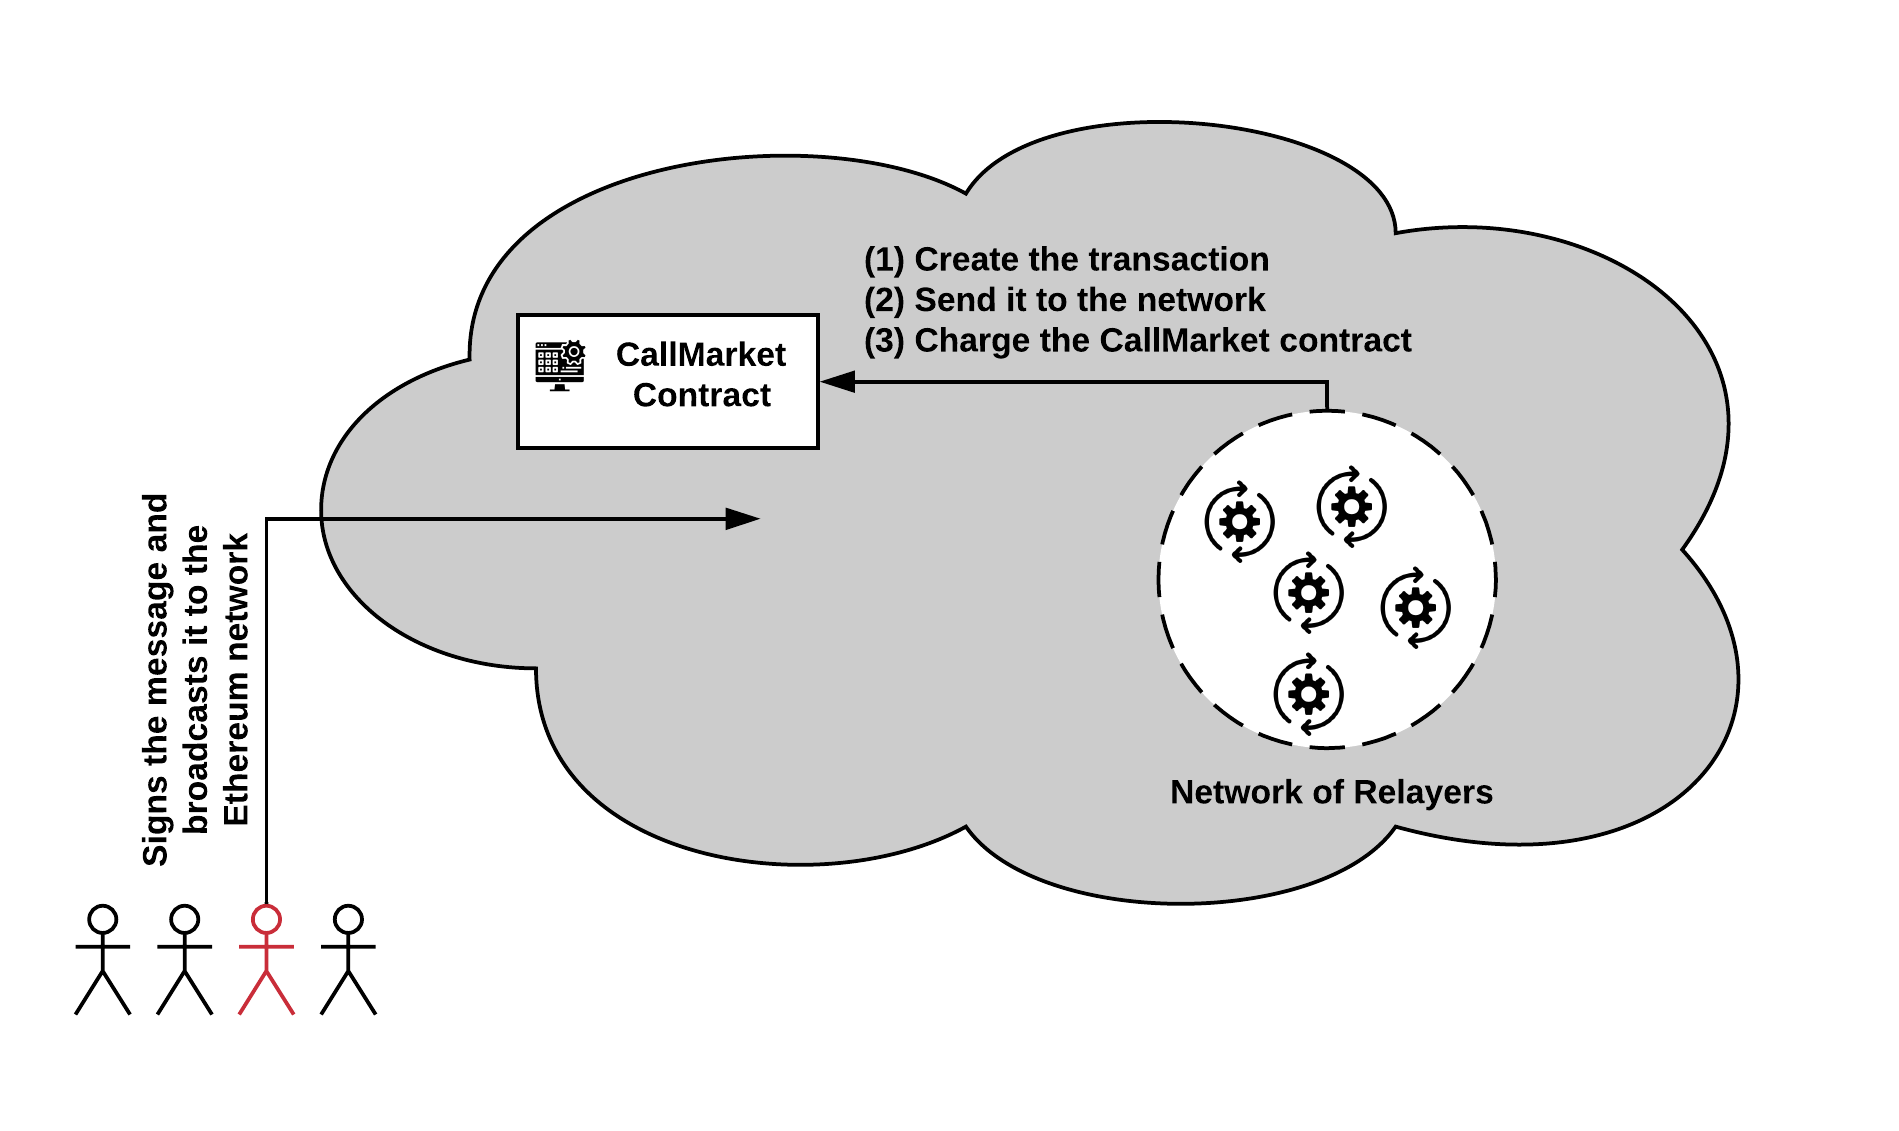
\includegraphics[width=0.8\textwidth]{fig/meta_tx.png}
\caption{\footnotesize{}  \label{fig:meta_tx}}
\end{figure}

% = = = = = = = = = = = = = = = = = = = = = = = = = = = = = = = = = %

%= = = = = =  = =  =  Users close and get refunded with the contract funds (collected as fees during order submissions) =  = = = = = = = = =%

\item \textbf{Using the "Contract Pays" Model.} An alternative solution is to design the market such that the last person to submit an order calls the \texttt{CloseMarket()} function, but in contrast to a normal transaction (where the person initiating the transaction must pay the fee), here the CallMarket contract pays the cost for closing the market and matching the orders respectively. To enforce this design we can use Solidity function modifiers; every time a new order is submitted, a function modifier checks whether (i) the auction period has to end and/or (ii) the maximum number of total orders has reached. If any of these two conditions are met, the \texttt{CloseMarket()} will be called. Again, market participants are charged with certain amounts of fees every time they submit an order, these fees are accumulated in the CallMarket. Once the \texttt{CloseMarket()} is successfully executed and orders are matched, the contract transfers its funds to that person. Note that here the person must still have enough gas to cover the execution of the transaction as the funds will be only transferred after the transaction is fully executed. However, market participants are incentivized to do so as they may receive more ethers than they have spent.

%= = = = = =  = =  =  Rollups=  = = = = = = = = =%

\item \textbf{Using Rollups.} Rollup is a scaling method that moves the storage and computation of the smart contracts off-chain while maintaining the transaction data on the main chain as call-data. In this technique, any Ethereum user can act as a validator; they can execute the \texttt{CloseMarket()}function and only post the new state of the contract (the updated balance of traders) in the form of \textit{assertions} to the main chain. Rollups improve scalability, provide faster and cheaper execution of the contracts, and eliminate the gas limit as the contract is no longer executed on-chain.
In the followings we briefly discuss different rollup proposals and techniques. Each approach uses a different method to ensure correction of assertions:


\begin{itemize}

\item \textbf{{Non-interactive Rollups.}} In this rollup technique, assertions are posted together with a validity proof that would be later used by validators to check if the \texttt{CloseMarket()} function has been executed correctly. ZK-Rollup scheme is one of the solutions that uses ZK-SNARKs to prove the validity of the assertions in zero-knowledge. ZK proofs are quick and cheap to verify but they are expensive and time consuming to generate. These proofs could be generated (i) for free or (ii) the CallMarket contract could collect proportional fees for every trade that is successfully executed.

\item \textbf{{Optimistic Rollups.}} In this scheme, assertions are assumed to be valid if there is no dispute posted about them with a certain window of time (a.k.a. "the challenge period'). Here, dispute resolution is a gas-costly method as the CallMarket contract would have to emulate the transaction on-chain to ensure the correctness the assertion. This scheme introduces a tradeoff between privacy and performance as all the assertions are publicly available and accessible. However, here the new state only reflects the updated balances of traders and no secret is involved. 

\item \textbf {{Multi-round Interactive Rollups.}} In this design paradigm, \textit{pending assertions} are posted on-chain and they are open to dispute. Once the challenge period is over and no challenge is submitted, the assertion is confirmed and the CallMarket contract transitions to the new state (\ie updates traders' balances). This scheme takes the overhead for the CallMarket contract to execute the \texttt{Close()} on-chain by using rounds to the dispute resolutions. The two parties (asserter and challenger) must run an interactive protocol and the CallMarket smart contract would have to act as a referee and decides which party's claim is true. Arbitrum is an example of multi-round interactive rollups that uses an efficient challenge-based protocol to penalize the dishonest parties~\cite{kalodner2018arbitrum}. 

\end{itemize}

%= = = = = =  = =  =  SGX=  = = = = = = = = =%

\item \textbf{{Using Trusted Execution Environments.}} Another way of achieving execution of the \texttt{CloseMarket()} function is incorporating the Ethereum blockchain into the Trusted Execution Environments (TEEs) and decoupling the contract execution from consensus mechanism. TEEs enable secure execution of applications in an isolated processing environment called the \textit{enclave}. Here, the enclave could execute the \texttt{CloseMarket()} function off-chain in TEEs and publish an on-chain attestation Quote to the CallMarket contract. The contract then verifies the correctness of the Quote and if validated correctly, it transitions to the new state. Ekiden is an example that uses Intel SGX to solve the scalability and confidentiality issues with the smart contract execution~\cite{cheng2019ekiden}. A drawback of this scheme is in order to achieve confidentiality-preserving smart contracts we have to trust a trusted party in the form of the hardware manufacturer (\eg Intel).


\end{enumerate}


% = = = = = = = = = = = = = = = = = = = = = = = = = = = = = = = = = = = = = = = = = = = = = = = = = = = = = = = = = = = = = = = = = = = = =  %



% = = = = = = = = = = = =Uint testing the PQs Table = = = = = = = = = = = = =  %

\section{Unit Testing the Priority Queues}

Here we execute the same JavaScrip test on the five priority queues with an end goal of unit testing them. We enter 50 unsigned integers to the priority queues in random ordering. To do so, we use JavaScript \texttt{Math.random()} function to generate pseudo-random integers between 1 and 200. Figure~\ref{fig:average_uints_insertion} shows the gas cost variations for entering 50 unsigned integers in the five data structures. The x-axis is the place in line (\eg the10th number entered in the priority queue) and the and y-axis is the cost of that transaction in gas. 

% = = = = = = = = = = = =average_uints_insertion Figure = = = = = = = = = = = = =  %

\begin{figure}[htb!p]
\centering
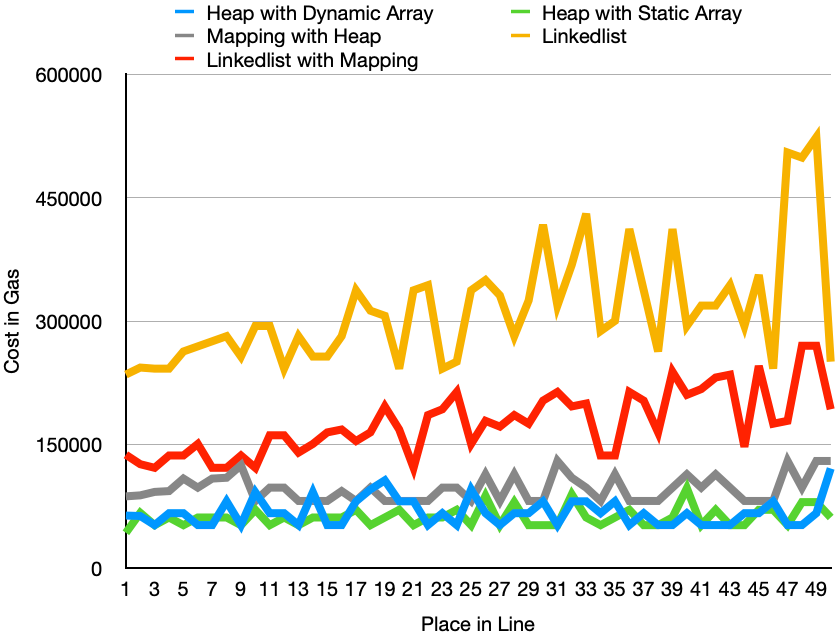
\includegraphics[width=1\textwidth]{fig/average_uints_insertion.png}
\caption{\footnotesize{}  \label{fig:average_uints_insertion}}
\end{figure}

% = = = = = = = = = = = = = = = = = = = = = = = = = = = = = = = = = = = = = = = =  %

Then, we call the \texttt{Dequeue()} function which iteratively removes the maximum value of the priority queue (until the data structure is empty). The computational costs for dequeuing 50 unsigned integers in each priority queue are outlined in Table~\ref{tab:PQ_UnitTests}. The tests are performed using the current Ethereum gas metrics (block gas limit $=$11,741,495 and 1 gas $=$ 56 gwei)~\footnote{https://ethstats.net/}. The second column of the table shows the net gas consumption (the gasUsed value derived from transaction receipts) for removing 50 integers from each priority queues.  

At the time of this writing, Ethereum transaction receipts only contain the net gas consumption and not the total gas consumption ( total gas consumption is defined as $gas refunded + gasUsed$ ) and we cannot find out the value of the EVM's refund counter from inside the EVM.

So in order to account for refunds inside each priority queue smart contract, we can calculate them manually; first we figure out exactly how much storage is being cleared when dequeuing  the max integers and then we could multiply the number of storage slots cleared by 15,000 (see the last column of Table~\ref{tab:PQ_UnitTests}).

Another way to know the amount of refund in each priority queue is to use the \texttt{estimateGas API} which provides a rough idea about the total amount of gas that is required for a transaction to go through. The \texttt{web3.eth.estimateGas} pretends the transaction is included in the block and its functions (with the parameters passed) will be executed on the Ethereum blockchain. Doing so, it provides us an estimate of how much gas is needed to be sent with the transaction. The second and third columns of Table~\ref{tab:PQ_UnitTests}) show the total amount of gas required for dequeuing 50 integers from each priority queue (provided by estimateGas) and the amount of gas refund ($Total Gas Consumption - gasUsed$) respectively.

Note that in order to urge miners to process smart contract with refunds, the accumulated gas refund can never exceed half the gas used up during computation~\cite{wood2014ethereum}. So at the end of a successful transaction, the amount of gas in the refund counter (capped at half the net gas used) is returned to the caller. For example, the amount of gas that has been used when dequeuing 50 integers from the linkedlist with mapping data structure is 731,514 and since $3,000,000 > 731,514/2$, the amount of refund returned to the caller is $731,514/2 = 365,757$.

% = = = = = = = = = = = =Uint testing the PQs Table with 50 Random Integers between 1 and 200 = = = = = = = = = = = = =  %

\begin{table}[]
\centering
\begin{tabular}{|c|c|c|c|c|}
\hline

\textbf{\thead{Priority Queue}}    & \textbf{\thead{Net Cost\\in Gas}}      & \textbf{\thead{Total Cost\\in Gas\\(from estimateGas)}}      & \textbf{\thead{Gas Refund \\(from \texttt{estimateGas})}}    & \textbf{\thead{Gas Refund \\(Manually Calculated)}} \\ \hline

% = = = = = = = = = = = = = = = = = = = = = = = = = = = = = = = = = = = = = = = = = = = = = = = = = = = = = = = = = = = = = = = = = = = = = = %
	\textbf{\thead{Heap with \\ Dynamic Array}}         				& 2,575,997               & 3,349,746		& 773,749             & 750,000                       \\ \hline
% = = = = = = = = = = = = = = = = = = = = = = = = = = = = = = = = = = = = = = = = = = = = = = = = = = = = = = = = = = = = = = = = = = = = = = %
	\textbf{\thead{Heap with \\ Static Array}}           				& 1,324,856                & 2,090,182     	& 765,326             & 750,000                      \\ \hline
% = = = = = = = = = = = = = = = = = = = = = = = = = = = = = = = = = = = = = = = = = = = = = = = = = = = = = = = = = = = = = = = = = = = = = = %
	\textbf{\thead{Mapping with \\ keys stored \\ in Heap}} 		& 2,863,239                & 4,378,584       	& 1,515,345           & 1,500,000                     \\ \hline
% = = = = = = = = = = = = = = = = = = = = = = = = = = = = = = = = = = = = = = = = = = = = = = = = = = = = = = = = = = = = = = = = = = = = = = %
	\textbf{Linkedlist}                       							& 557,085               	& 1,772,085      	& 1,215,000           & 1,200,000                      \\ \hline
% = = = = = = = = = = = = = = = = = = = = = = = = = = = = = = = = = = = = = = = = = = = = = = = = = = = = = = = = = = = = = = = = = = = = = = %
	\textbf{\thead{Linkedlist with \\ Mapping}}          				& 731,514              	& 3,731,514       	& 3,000,000     	  &  3,765,000                       \\ \hline
% = = = = = = = = = = = = = = = = = = = = = = = = = = = = = = = = = = = = = = = = = = = = = = = = = = = = = = = = = = = = = = = = = = = = = = %

\end{tabular}
\caption{\footnotesize{PQUnitTests with 50 Random Integers between 1 and 200}
\label{tab:PQUnitTests_random}}
\end{table}
% = = = = = = = = = = = = = = = = = = = = = = = = = = = = = = = = = = = = =  %



% = = = = = = = = = = = =Uint testing the PQs Table with 50 Integers (NOT RANDOM!) = = = = = = = = = = = = =  %

\begin{table}[]
\centering
\begin{tabular}{|c|c|c|c|c|}
\hline

\textbf{\thead{Priority Queue}}    & \textbf{\thead{Net Cost\\in Gas}}      & \textbf{\thead{Total Cost\\in Gas\\(from estimateGas)}}      & \textbf{\thead{Gas Refund \\(from \texttt{estimateGas})}}    & \textbf{\thead{Gas Refund \\(Manually Calculated)}} \\ \hline

% = = = = = = = = = = = = = = = = = = = = = = = = = = = = = = = = = = = = = = = = = = = = = = = = = = = = = = = = = = = = = = = = = = = = = = %
	\textbf{\thead{Heap with \\ Dynamic Array}}         				& 2,394,202                & 3,159,551           &765,349	    & 750,000                     \\ \hline
% = = = = = = = = = = = = = = = = = = = = = = = = = = = = = = = = = = = = = = = = = = = = = = = = = = = = = = = = = = = = = = = = = = = = = = %
	\textbf{\thead{Heap with \\ Static Array}}           				& 1,317,922                & 2,083,240   	& 765,318          & 750,000                     \\ \hline
% = = = = = = = = = = = = = = = = = = = = = = = = = = = = = = = = = = = = = = = = = = = = = = = = = = = = = = = = = = = = = = = = = = = = = = %
	\textbf{\thead{Mapping with \\ keys stored \\ in Heap}} 		& 2,629,191                & 4,144,536       	&1,515,345          & 1,500,000                     \\ \hline
% = = = = = = = = = = = = = = = = = = = = = = = = = = = = = = = = = = = = = = = = = = = = = = = = = = = = = = = = = = = = = = = = = = = = = = %
	\textbf{Linkedlist}                       							&557,085            		& 1,772,085      	&1,215,000          & 1,200,000                      \\ \hline
% = = = = = = = = = = = = = = = = = = = = = = = = = = = = = = = = = = = = = = = = = = = = = = = = = = = = = = = = = = = = = = = = = = = = = = %
	\textbf{\thead{Linkedlist with \\ Mapping}}          				&731,514              	&3,731,514      	& 3,000,000    	  &  3,765,000                       \\ \hline
% = = = = = = = = = = = = = = = = = = = = = = = = = = = = = = = = = = = = = = = = = = = = = = = = = = = = = = = = = = = = = = = = = = = = = = %

\end{tabular}
\caption{\footnotesize{PQUnitTests}
\label{tab:PQ_UnitTests}}
\end{table}
% = = = = = = = = = = = = = = = = = = = = = = = = = = = = = = = = = = = = =  %


%============= Experiments =================== %
\section{Experiments}

Our application was developed in Solidity using the Truffle development framework and deployed on Ganache-CLI. We used Javascript for testing by leveraging the Mocha testing framework. Followings outline the results of different tests we performed.

%============= Test 1 (17_Worst_Case_Matching_test.js) Tables=================== %

 \subsection{Experiments on the \texttt{Match()} Function}

We executed the same test on the the five different versions of the CallMarket we implemented using five priority queues to examine the cost of the \texttt{Match()} function as well as the maximum pairs of bid and ask orders it can handle in each case. The \texttt{Match()} function's computational cost and the maximum number of orders it can execute in each case (before running out of gas) are outlined in Table~\ref{tab:worst_case_matching}. Note that this is a \textit{worst case matching} test where all bids and asks are submitted as marketable limit orders with specified prices that would be filled undoubtedly, performed using the current Ethereum gas metrics (block gas limit $=$11,741,495 and 1 gas $=$ 56 gwei)~\footnote{https://ethstats.net/}. The last column of Table~\ref{tab:worst_case_matching} shows the gas cost of matching 1000 pairs of bids and asks for each priority queue for which we set the block gas limit to the maximum of  $2^{53}$ (the Javascript's max safe integer).

% gas sent with each transaction here is 11,000,000
%======= estimateGas() function = gasUsed + gasRefund =======%

% Heap with Dynamic Array: match.estimateGas() = 7204994 => gasRefund = 7204994 - 3274994 = 3930000
% Heap with Static Array: match.estimateGas() = 7337527 => gasRefund = 7337527 - 3107527 = 4230000
% Mapping with keys stored in Heap: match.estimateGas() = 6644803 => gasRefund = 6644803 - 5414803 = 1230000
% Linkedlist: match.estimateGas() = 7629847 => gasRefund = 7629847 -  3279847 = 4350000
% Linkedlist with Mapping: match.estimateGas() = 7227717 => gasRefund = 7227717 -  3297717 = 3930000

%===============================================%


% = = = = = = = = = = = =Worst_Case_Matching Table = = = = = = = = = = = = =  %

\begin{table}[]
\centering
\begin{tabular}{|c|c|c|c|}
\hline

\textbf{\thead{Priority Queue}}    & \textbf{\thead{Maximum Number \\ of \\ Matched Orders}}      & \textbf{\thead{Net Cost\\in Gas}}          & \textbf{\thead{Net Cost in Gas\\ for \\ 1000 Pairs \\ of Orders}} \\ \hline

% = = = = = = = = = = = = = = = = = = = = = = = = = = = = = = = = = = = = = = = = = = = = = = = = = = = = = = = = = = = = = = = = = = = = = = %
	\textbf{\thead{Heap with \\ Dynamic Array}}         				& 38 pairs                & 5,372,679                   	& 457,326,935                      \\ \hline
% = = = = = = = = = = = = = = = = = = = = = = = = = = = = = = = = = = = = = = = = = = = = = = = = = = = = = = = = = = = = = = = = = = = = = = %
	\textbf{\thead{Heap with \\ Static Array}}           				& 42 pairs                & 5,247,636                  	& 333,656,805                       \\ \hline
% = = = = = = = = = = = = = = = = = = = = = = = = = = = = = = = = = = = = = = = = = = = = = = = = = = = = = = = = = = = = = = = = = = = = = = %
	\textbf{\thead{Mapping with \\ keys stored \\ in Heap}} 		& 46 pairs                & 5,285,275                     & 226,499,722                        \\ \hline
% = = = = = = = = = = = = = = = = = = = = = = = = = = = = = = = = = = = = = = = = = = = = = = = = = = = = = = = = = = = = = = = = = = = = = = %
	\textbf{Linkedlist}                       							& 152 pairs                & 5,495,265                     & 35,823,601                        \\ \hline
% = = = = = = = = = = = = = = = = = = = = = = = = = = = = = = = = = = = = = = = = = = = = = = = = = = = = = = = = = = = = = = = = = = = = = = %
	\textbf{\thead{Linkedlist with \\ Mapping}}          				& 86 pairs                 & 5,433,259                     & 62,774,170                        \\ \hline
% = = = = = = = = = = = = = = = = = = = = = = = = = = = = = = = = = = = = = = = = = = = = = = = = = = = = = = = = = = = = = = = = = = = = = = %

\end{tabular}
\caption{\footnotesize{}
\label{tab:worst_case_matching}}
\end{table}



%%============= Test 3 (17_Worst_Case_Submission_test.js) Figures==================== %
%
% \subsection{Experiments on \texttt{Submit Order()} Functions}
%
%We executed another set of tests on the the five different versions of the CallMarket in which we sent 200 \texttt{SubmitBid} to the CallMarket to simulate two hundred of traders participating in the market. These tests were performed in two levels (i) worst case and (ii) average case submissions. 
%%the data structure used for bids and asks is the same and hence the submission plots for 200 submitbids and 200 submitasks. Do we have to mention that here?
%
%% = = = = = = = = = = = =Worst_Case_Submission = = = = = = = = = = = = =  %
%
%\subsubsection{Worst Case Order Submission}
%
%Here each \texttt{SubmitBid()} transaction has a price that is smallest or second-smallest of the transactions after it. Doing so, we ensure all the orders move every time a new order is sent to the market. Figure~\ref{fig:worst_case_submission} shows the gas cost variations for submitting 200 orders in five versions of the CallMarket. The x-axis is the place in line (\eg the 10th person to submit the order) and the and y-axis is the gas cost for sending that transaction.
%
%%And conversely each \texttt{SubmitAsk()} transaction has a price that is biggest or second-biggest of the transactions after it
%
%% = = = = = = = = = = = =Worst_Case_Submission Figure = = = = = = = = = = = = =  %
%
%\begin{figure}[htb!p]
%\centering
%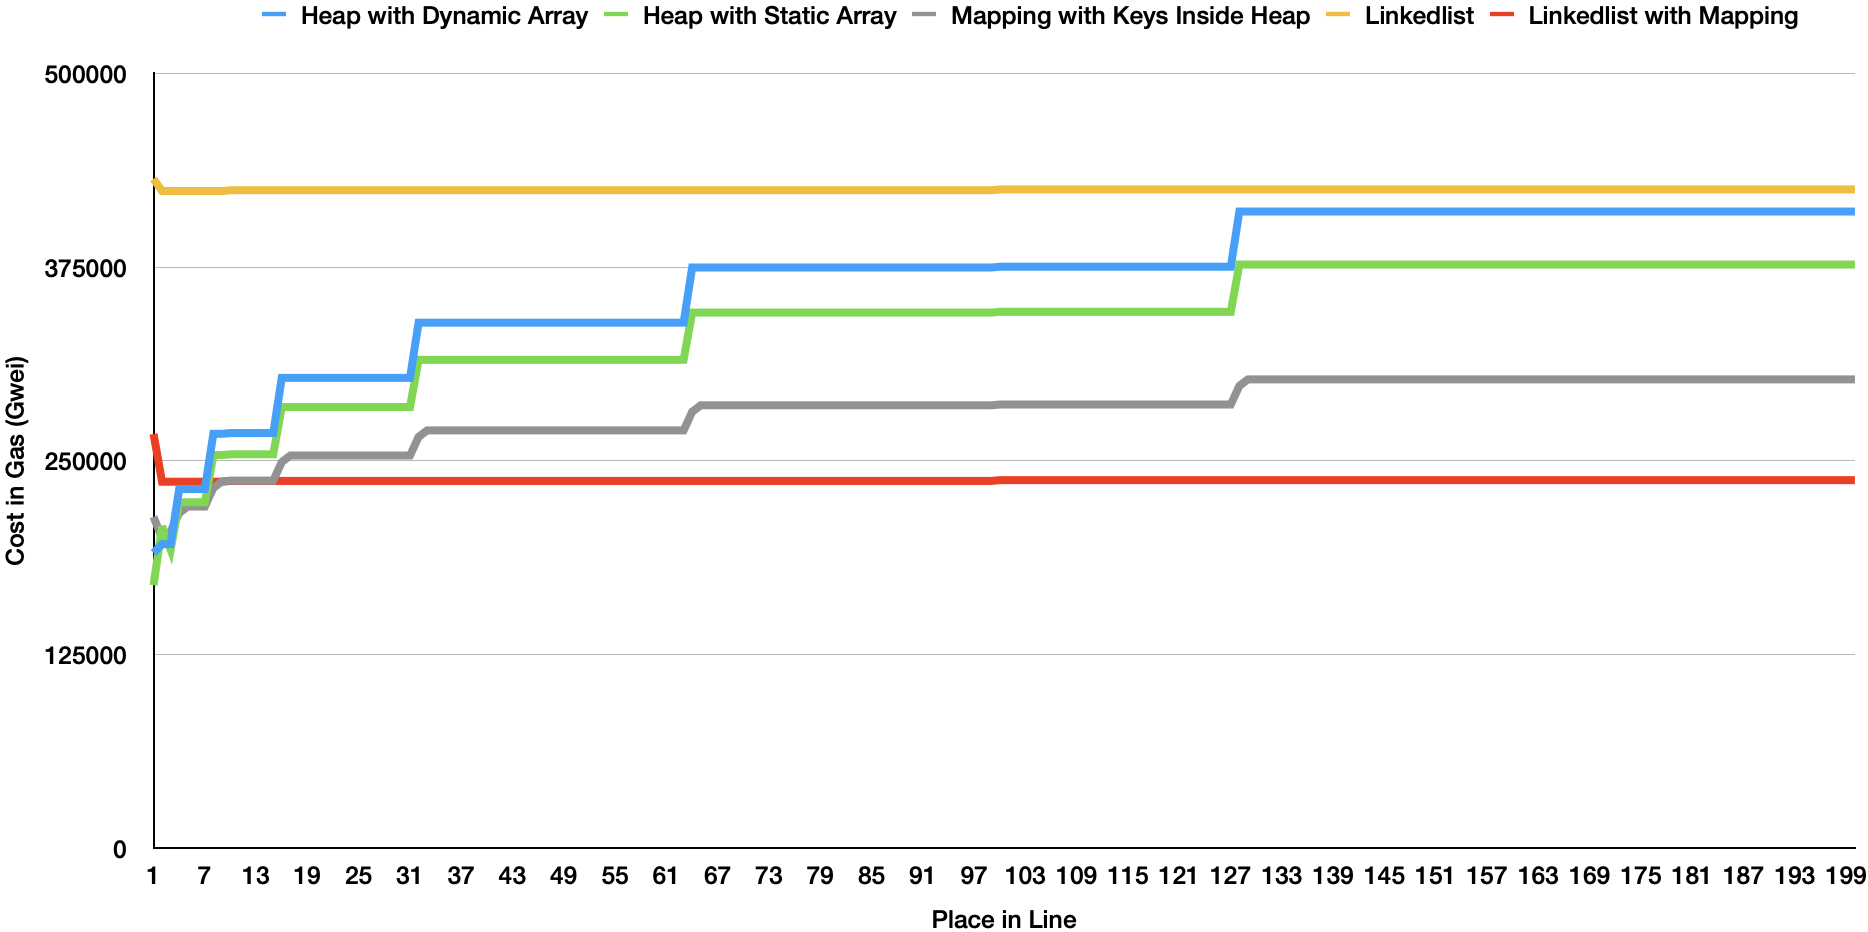
\includegraphics[width=1\textwidth]{fig/worst_case_submission_3.png}
%\caption{\footnotesize{}  \label{fig:worst_case_submission}}
%\end{figure}
%
%% = = = = = = = = = = = = = = = = = = = = = = = = = = = = = = = = = = = = = = = =  %
%
%
%% = = = = = = = = = = = =Average_Case_Submission = = = = = = = = = = = = =  %
%
%\subsubsection{Average Case Order Submission}
%
%Here we test the five versions of the CallMarket when 200 bid orders are entered in random ordering. To do so, we use JavaScript \texttt{Math.random()} function to generate pseudo-random integers between 1 and 100. Figure~\ref{fig:average_case_submission} shows the gas cost variations for submitting 200 orders in five versions of the CallMarket. Again the x-axis is the place in line (\eg the10th person to submit the order) and the and y-axis is the gas cost for submitting that transaction. 
%
%% = = = = = = = = = = = =Average_Case_Submission Figure = = = = = = = = = = = = =  %
%
%\begin{figure}[htb!p]
%\centering
%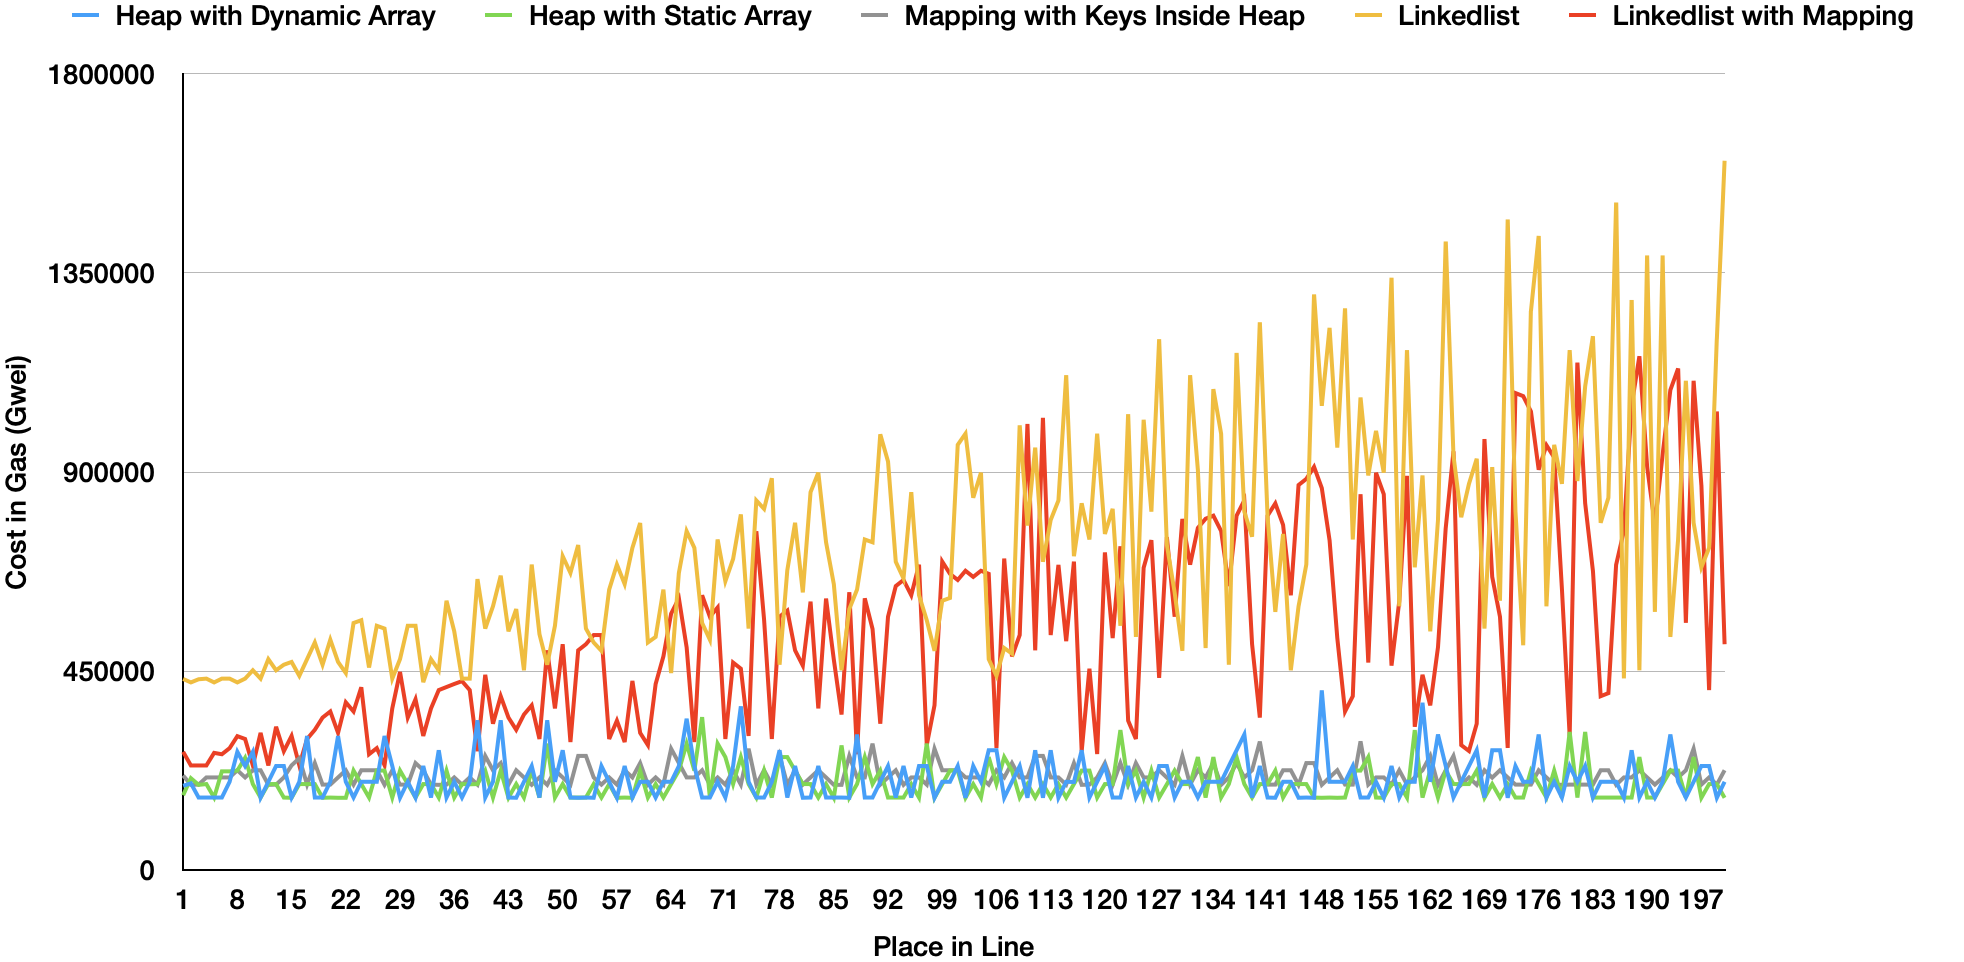
\includegraphics[width=1\textwidth]{fig/average_case_submission_3.png}
%\caption{\footnotesize{}  \label{fig:average_case_submission}}
%\end{figure}
%
%% = = = = = = = = = = = = = = = = = = = = = = = = = = = = = = = = = = = = = = = =  %














%======================================== %

% = = = = = = = = = = = = = = = = = = = = = = = = = = = = = = = = = = = = = = = = = =

\section{Concluding Remarks}


 
%\subsubsection*{Acknowledgements.} J. Clark thanks ...

































